\level{2}{Norris}

	\begin{figure}[H]\centering
        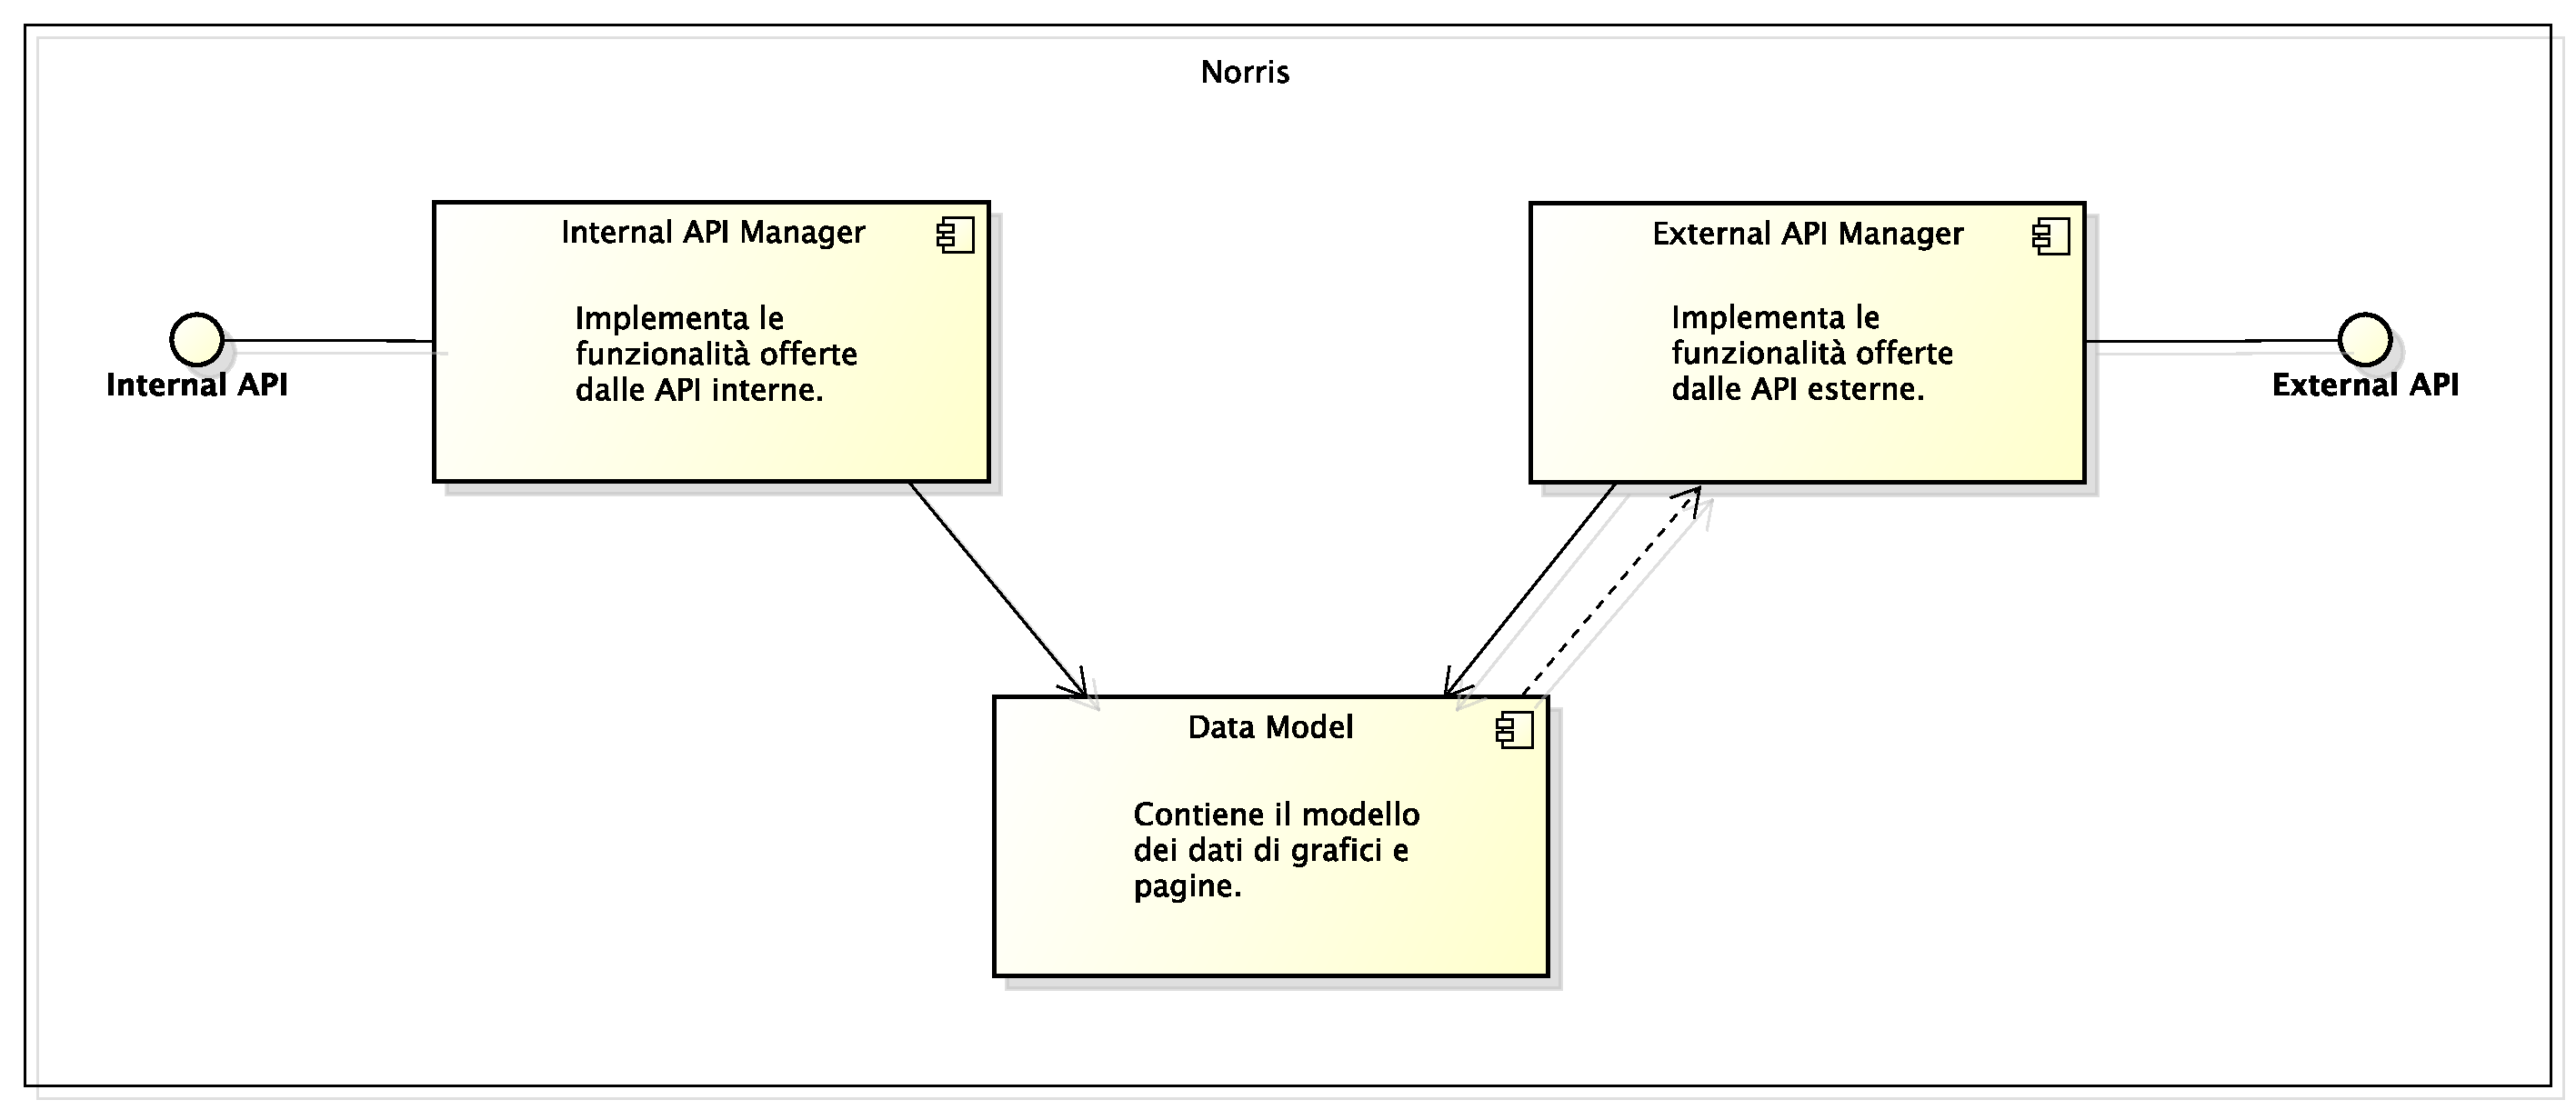
\includegraphics[width=\textwidth]{SpecificaTecnica/Pics/ComponentiNorris}
        \caption{Diagramma delle componenti di Norris}
    \end{figure}


    \level{3}{Descrizione delle componenti di Norris}

    	\level{4}{Internal API Manager}
			La componente Internal API Manager rappresenta un controller per le API interne. Essa si occupa di implementare le funzionalità offerte dall'interfaccia delle API interne, ovvero:
			\begin{itemize}
				\item creare un'istanza di Norris;
				\item creare nuovi grafici;
				\item aggiornare i grafici;
				\item creare nuove pagine;
				\item aggiungere i grafici all'istanza di Norris;
				\item aggiungere le pagine all'istanza di Norris;
				\item aggiungere i grafici alle pagine;
				\item scegliere le impostazioni relative a grafici, pagine e istanza;
				\item permette la definizione di funzioni per l'autenticazione.
			\end{itemize}
		Questa componente si occupa, inoltre, di generare in automatico le pagine create all'interno di un'istanza di Norris, a partire dai modelli in essa contenuti.

		\level{4}{Data Model}
			La componente Data Model è un modello che astrae un'istanza di Norris. Al suo interno vi sono le informazioni relative alla struttura di grafici e pagine, assieme alle rispettive impostazioni. Inoltre vengono fissate le regole con le quali grafici e pagine vengono composti assieme per formare un'istanza di Norris. Il Data Model fornisce i metodi per inserire i dati e configurare le impostazioni. Fornisce inoltre dei metodi per ottenere i valori di queste ultime, in modo da poterle riutilizzare per un altro grafico o pagina. Infine, è qui che vengono memorizzate le informazioni inerenti l'autenticazione.

		\level{4}{External API Manager}
			La componente External API Manager rappresenta un controller per le API esterne. Essa implementa le funzionalità offerte dall'interfaccia delle API esterne, ovvero:
			\begin{itemize}
				\item ottenere la lista dei grafici;
				\item ottenere un grafico con relativi aggiornamenti;
				\item effettuare il login;
				\item effettuare il logout.
			\end{itemize}
		Questa componente si occupa, inoltre, di gestire la comunicazione con il server web. Gestisce quindi sia le richieste HTTP, sia la comunicazione tramite un canale websocket.

	\level{3}{Descrizione delle interazione tra le componenti}

		\level{4}{Internal API Manager - Data Model}
			Quando lo sviluppatore richiama una funzione definita dalle API interne, la componente Internal API Manager effettua le opportune operazioni di lettura/scrittura nel Data Model.

		\level{4}{External API Manager - Data Model}
			Per fornire le funzionalità descritte dalle API esterne, la componente External API Manager interroga il Data Model sullo stato attuale dell'istanza, richiedendo le informazioni in esso contenute.

		\level{4}{Data Model - External API Manager}
			Quando avviene una modifica nel Data Model, una notifica avvisa l'External API Manager di un avvenuto cambiamento nel modello dei dati. In particolare External API Manager viene notificato quando viene creato un nuovo grafico o quando un grafico esistente viene aggiornato.
